\let\negmedspace\undefined
\let\negthickspace\undefined
\documentclass[journal]{IEEEtran}

\usepackage[a5paper, margin=10mm, onecolumn]{geometry}
%\usepackage{lmodern} % Uncomment if needed for pdflatex
\usepackage{tfrupee} % Include tfrupee package

\setlength{\headheight}{1cm} % Set the height of the header box
\setlength{\headsep}{0mm}     % Set the distance between the header box and the top of the text

\usepackage{gvv-book}
\usepackage{gvv}
\usepackage{cite}
\usepackage{amsmath,amssymb,amsfonts,amsthm}
\usepackage{algorithmic}
\usepackage{graphicx}
\usepackage{textcomp}
\usepackage{txfonts}
\usepackage{listings}
\usepackage{enumitem}
\usepackage{mathtools}
\usepackage{gensymb}
\usepackage{comment}
\usepackage[breaklinks=true]{hyperref}
\usepackage{tkz-euclide} 
\usepackage{inputenc}                                        
\usepackage{color}                                            
\usepackage{array}                                            
\usepackage{longtable}                                       
\usepackage{calc}                                             
\usepackage{multirow}                                         
\usepackage{hhline}                                           
\usepackage{ifthen}                                           
\usepackage{lscape}
\usepackage{tikz}
\usepackage{circuitikz}
\usepackage{standalone} % For including external TikZ files
\usepackage{longtable}

\begin{document}

\bibliographystyle{IEEEtran}
\vspace{3cm}

\title{Scientific Calculator}
\author{EE24BTECH11066 - YERRA AKHILESH}
\maketitle

\renewcommand{\thefigure}{\theenumi}
\renewcommand{\thetable}{\theenumi}
\setlength{\intextsep}{10pt} % Space between text and floats

\numberwithin{equation}{enumi}
\numberwithin{figure}{enumi}
\renewcommand{\thetable}{\theenumi}

\section{Connections}
\subsection{ Connecting the LCD Display (Left to Right Order)}

The 16x2 LCD is interfaced with the Arduino using the 4-bit mode connection as follows:

\begin{table}[h!]
\centering
\begin{tabular}{|c|c|}
\hline
\textbf{LCD Pin} & \textbf{Connected to Arduino Pin} \\
\hline
VSS & GND \\
VDD & 5V \\
VO & Middle Pin of Potentiometer \\
RS & Digital Pin 1 \\
RW & GND \\
E & Digital Pin 0 \\
D0 &  (Not Connected) \\
D1 &  (Not Connected) \\
D2 &  (Not Connected) \\
D3 &  (Not Connected) \\
D4 & Digital Pin 5 \\
D5 & Digital Pin 4 \\
D6 & Digital Pin 3 \\
D7 & Digital Pin 2 \\
A (LED+) & 5V \\
K (LED-) & GND \\
\hline
\end{tabular}
%\caption{LCD Pin to Arduino Pin Mapping}
\end{table}

\textbf{Potentiometer Wiring:}
\begin{itemize}
  \item Leftmost Pin $\rightarrow$ GND
  \item Middle Pin $\rightarrow$ LCD VO (Contrast Pin)
  \item Rightmost Pin $\rightarrow$ 5V
\end{itemize}
\begin{figure}[h!]
   \centering
   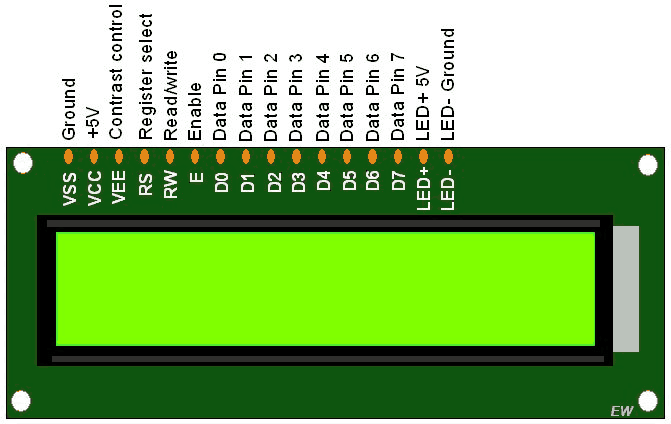
\includegraphics[width=0.50\columnwidth]{figs/LCD.png}
   \label{stemplot}
\end{figure}

\subsection{Connecting the Input Buttons }

Each button is connected in pull-up mode, meaning:
\begin{itemize}
  \item One terminal of each button goes to an Arduino input pin.
  \item The other terminal is connected to GND.
\end{itemize}

\begin{table}[H]
\centering
\begin{tabular}{|c|c|}
\hline
\textbf{Button Function} & \textbf{Connected to Arduino Pin} \\
\hline
Number 0 & Digital Pin 13 \\
Number 1 & Digital Pin 12 \\
Number 2 & Digital Pin 11 \\
Number 3 & Digital Pin 10 \\
Number 4 & Digital Pin 9 \\
Number 5 & Digital Pin 8 \\
Number 6 & Digital Pin 7 \\
Number 7 & Digital Pin 6 \\
Number 8 & Analog Pin A0 \\
Number 9 & Analog Pin A1 \\
Operator Selection & Analog Pin A2 \\
Trigonometric Function & Analog Pin A3 \\
Reset Button & Analog Pin A4 \\
Enter (Evaluate Expression) & Analog Pin A5 \\
\hline
\end{tabular}
\end{table}
- \textbf{Each button’s other pin is connected to GND}

\subsection{Compiling and Uploading the Code}  
\vspace{0.3cm}  

\vspace{0.3cm}  
\subsubsection{ Compilation}   

\begin{verbatim}
avr-gcc -mmcu=atmega328p -DF_CPU=16000000UL -Os -o scientific.elf scientific.c 
avr-objcopy -O ihex scientific.elf scientific.hex
\end{verbatim}  

\vspace{0.3cm}  
\subsubsection{Uploading part}  
\begin{verbatim}
sudo avrdude -c arduino -P /dev/ttyACM0 -b 115200 -p atmega328p -U flash:w:scientific.hex
\end{verbatim}  

\vspace{0.3cm}  
Ensure that the microcontroller is connected to the correct port (\texttt{/dev/ttyACM0}) before executing the upload command.  
\vspace{0.5cm}  


\section{Main Features}
\begin{itemize}
    \item \textbf{LCD Display (4-bit Mode)}: Uses a 4-bit connection to show numbers and results.
    \item \textbf{14 Buttons for Input}: Includes 10 number buttons (0-9), a decimal point button, an operator selection button, a trigonometric function button, and an enter button.
    \item \textbf{Basic Math Operations}: Supports addition ($+$), subtraction ($-$), multiplication ($\times$), and division ($\div$).
    \item \textbf{Trigonometric Functions}: Implements $\sin$, $\cos$, $\tan$, and their inverse functions ($\sin^{-1}$, $\cos^{-1}$, $\tan^{-1}$).
    \item \textbf{Angle in Degrees}: Trigonometric calculations use degrees instead of radians.
    \item \textbf{Handles Long Calculations}: Supports multiple steps and follows operator precedence.
    \item \textbf{Error Detection}: Detects mistakes like division by zero and prevents incorrect calculations.
\end{itemize}

\section{How Buttons Work}
\subsection{Operator Button}
The arithmetic operator button cycles through different operations with each press:
\begin{enumerate}
    \item First press: Addition ($+$)
    \item Second press: Subtraction ($-$)
    \item Third press: Multiplication ($\times$)
    \item Fourth press: Division ($\div$)
    \item Fifth press: Returns to addition ($+$)
\end{enumerate}
The LCD displays the selected operator so the user knows the current choice.

\subsection{Trigonometric Function Button}
This button cycles through trigonometric functions in the following order:
\begin{enumerate}
    \item First press: $\sin$
    \item Second press: $\cos$
    \item Third press: $\tan$
    \item Fourth press: $\sin^{-1}$
    \item Fifth press: $\cos^{-1}$
    \item Sixth press: $\tan^{-1}$
    \item Seventh press: Returns to $\sin$
\end{enumerate}
The LCD displays the chosen function, allowing the user to input a value.

\section{How Code Works}
\subsection{Math Calculations}
\begin{itemize}
    \item Uses Taylor series for trigonometric calculations.
    \item Does not need extra math libraries.
    \item Checks if values for inverse trigonometric functions are valid.
\end{itemize}

\subsection{User Interface}
\begin{itemize}
    \item Single button selection for arithmetic and trigonometric functions.
    \item Button debouncing prevents multiple accidental inputs.
    \item The LCD clearly displays the current equation.
    \item Results are displayed with appropriate precision.
\end{itemize}

\subsection{Expression Calculation}
\begin{itemize}
    \item Correctly handles brackets and follows standard mathematical rules.
    \item Uses recursive parsing to evaluate complex expressions.
\end{itemize}

\subsection{Memory Usage}
\begin{itemize}
    \item Efficient storage for microcontroller use.
    \item Remembers the last result for continuous calculations.
\end{itemize}

\section{Special Features}
\begin{itemize}
    \item Supports floating-point calculations.
    \item Handles multi-step expressions correctly.
    \item Portable design for use with different hardware.
    \item Optimized for low-memory usage.
\end{itemize}

\section{Ease of Use}
\begin{itemize}
    \item Results can be used in further calculations.
    \item Single-button cycling makes operations simple.
    \item Prevents invalid inputs like multiple decimal points.
    \item Automatically fixes missing brackets in expressions.
\end{itemize}

\section{Final Summary}
This calculator is designed to be simple, efficient, and capable of handling complex calculations. It effectively manages memory and provides a smooth user experience, making it a great example of embedded system programming and mathematical implementation.

\begin{figure}[h!]
   \centering
   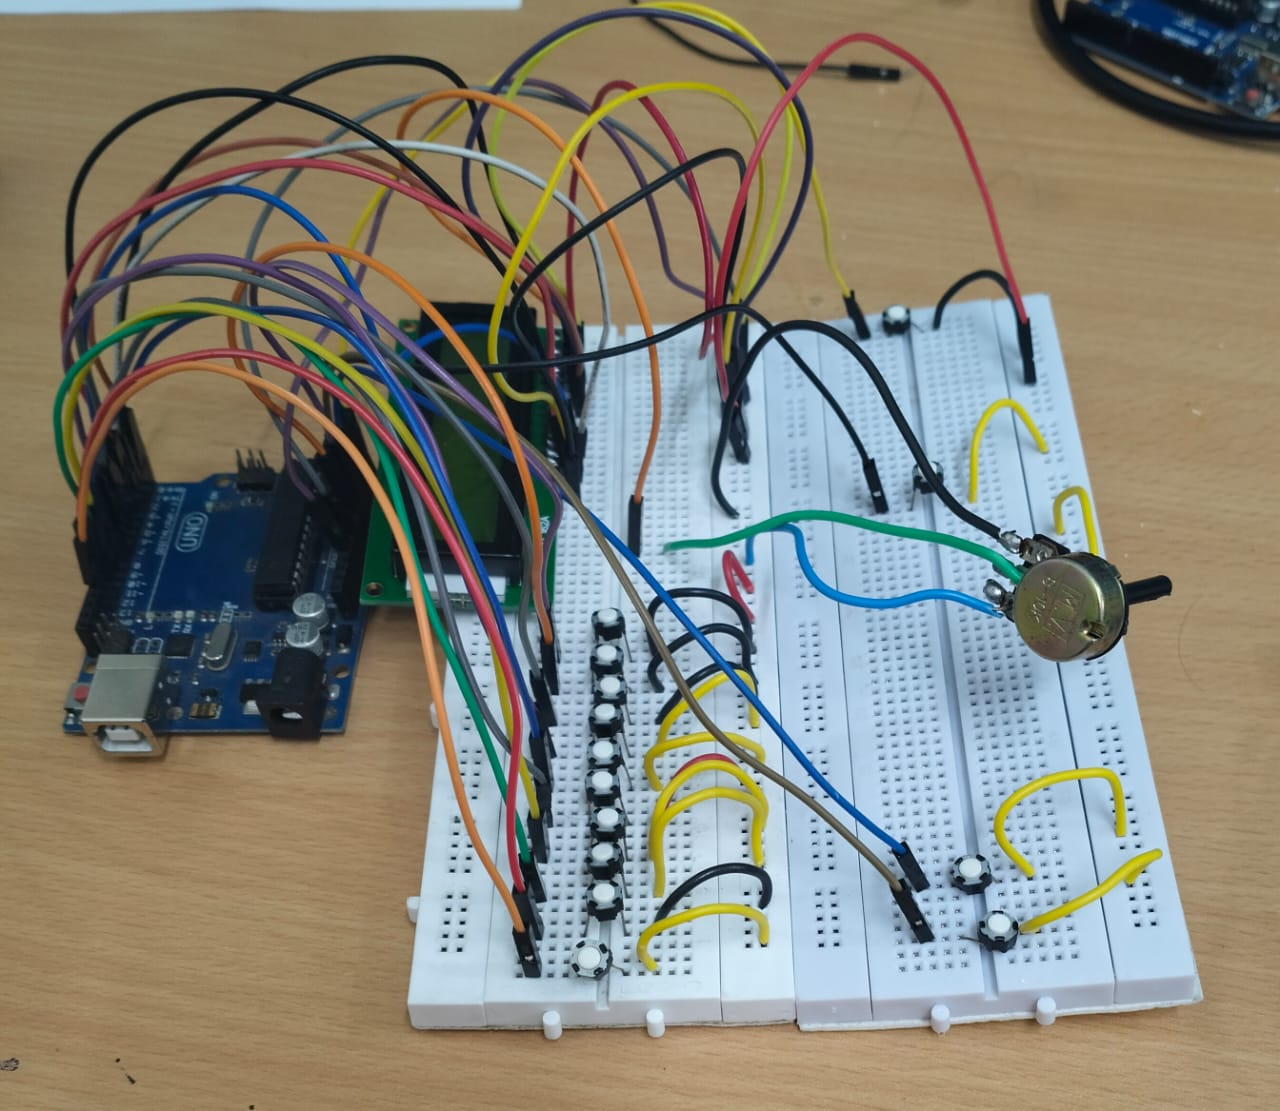
\includegraphics[width=0.50\columnwidth]{figs/Calculator_connections.jpeg}
   \label{stemplot}
\end{figure}
\end{document}

